\chapter{Ensemble Methods}
\label{cha:ensemble_methods}

\section{Ensemble Methods}

The rationale:
\begin{itemize}
	\item Groups of individuals can make better decisions than individuals (if
		they don't all think the same)

	\item Combining multiple ML models can produce better predictions than those of
		any single model

	\item Training ensembles can (often) be parallelized, with substantial
		computational savings
\end{itemize}

Models should be diverse enough for the ensemble to work. Ensembling strategies:

\begin{itemize}
	\item \textbf{bagging}: diversify the training sets

	\item \textbf{stacking}: diversify the models being trained

	\item \textbf{boosting}: (progressively) diversify the importance of examples
\end{itemize}

\section{Bagging: Bootstrap Aggregation}

\subsection{In a nutshell}
\begin{enumerate}[]
	\item Take a learning algorithm $\mathcal{A}$ (e.g. decision tree learning)

	\item Extract $m$ different datasets $\mathcal{D}^{(i)}$ from the original training
		set $\mathcal{D}$

	\item Train one base model per dataset
		\[
			f^{(i)}=\mathcal{A}\left(\mathcal{D}^{(i)}\right)
		\]

	\item Combine predictions of different base models
		\[
			\hat{y}=\operatorname{Combine}\left(f^{(1)}(x), \ldots, f^{(m)}(x)\right)
		\]
\end{enumerate}

\begin{figure}[H]
	\centering
	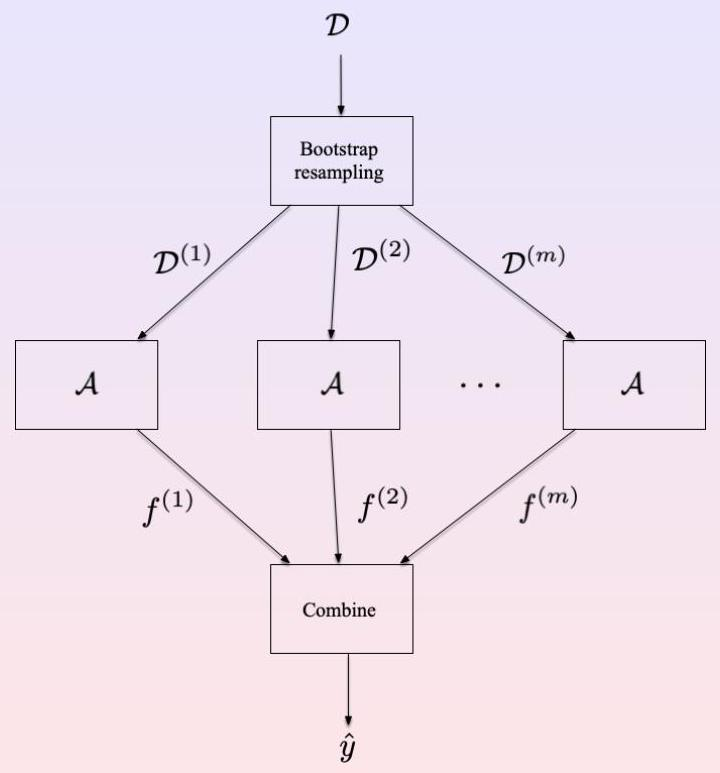
\includegraphics[scale=0.4]{
        images/17_EnsembleMethods_bagging.jpg
    }
	\caption{Bagging: Bootstrap aggregation}
\end{figure}

\subsection{Extracting Datasets: Boostrap Resampling}
Simply partitioning $\mathcal{D}$ into $m$ subsets produces very small training
sets. Bootstrap resampling extracts $N=|\mathcal{D}|$ samples from $\mathcal{D}$
with replacement (i.e., same example can be selected multiple times). Repeating
the procedure $m$ times to get diverse datasets of the same size as
$\mathcal{D}$.\\

\noindent
Diversity of Datasets:
\begin{itemize}
	\item Each example has probability $(1-1 / N)$ of not being selected at each draw

	\item Each example has probability $(1-1 / N)^{N}$ of not being selected after
		$N$ draws

	\item For large enough $N$, this is $37 \%$, i.e., $37 \%$ of the dataset are not
		part of a given training set (out-of-bag instances, oob)

	\item oob instances can be used to estimate test performance of the base model
\end{itemize}

\subsection{Combination Strategies}

Majority voting predict the class with most votes (classification)

\[
	\hat{y}=\operatorname{argmax}_{y}\sum_{i=1}^{m}\delta\left(y, \hat{y}^{(i)}\right
	)
\]

\noindent
Soft voting predict the class with largest sum of predicted probability (classification).
Assumes base classifier outputs a confidence/probability

\[
	\hat{y}=\operatorname{argmax}_{y}\sum_{i=1}^{m}f_{y}^{(i)}(x)
\]

\noindent
Mean predict the mean (or median) of the base model outputs (regression)

\[
	\hat{y}=\sum_{i=1}^{m}f^{(i)}(x)
\]

\subsection{Bagging example: Random forests}

Bagging and Model Decorrelation:
\begin{itemize}
	\item Use decision trees as the base models

	\item Even if $\mathcal{D}^{(i)}\neq \mathcal{D}^{(j)}$, the learned DTs can
		be too much correlated

	\item Introduce additional stochasticity in the DT training process

	\item At each node, choose the best feature to split from a random selection
		of the set of features (instead of using them all)
\end{itemize}

\section{Stacking: Stacked Generalization}

\subsection{In a nutshell}
\begin{enumerate}[]
	\item Train $m$ base models $f^{(i)}$ on $\mathcal{D}$ with $m$ different learning
		algorithms $\mathcal{A}^{(i)}$
		\[
			f^{(i)}=\mathcal{A}^{(i)}(\mathcal{D})
		\]

	\item Use a meta-learner to learn to combine base models (e.g., linear
		combination)
		\[
			g=\mathcal{A}_{\text{META }}\left(\left[f^{(1)}, \ldots, f^{(m)}\right], \mathcal{D}
			^{\prime}\right)
		\]

	\item Use the meta-model to output ensemble predictions
		\[
			\hat{y}=g\left(\left[f^{(1)}(x), \ldots, f^{(m)}(x)\right]\right)
		\]
\end{enumerate}

The meta-model should be trained on a dataset
$\mathcal{D}^{\prime}\neq \mathcal{D}$, or it will learn to focus on the best performing
model on $\mathcal{D}$.

\begin{figure}[H]
	\centering
	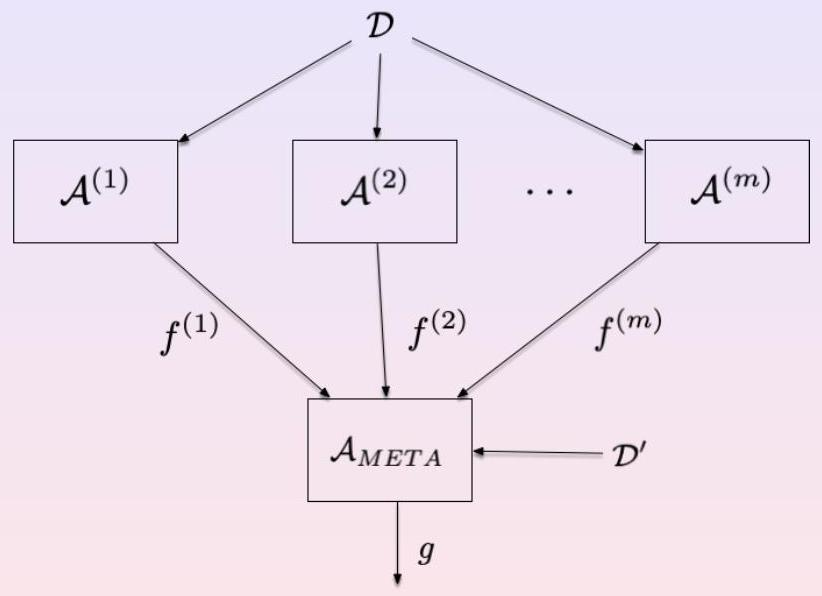
\includegraphics[scale=0.4]{
        images/17_EnsembleMethods_stacking.jpg
    }
	\caption{Bagging: Bootstrap aggregation}
\end{figure}

\section{Boosting}

\subsection{In a nutshell}
\begin{enumerate}[]
	\item Take a learner $\mathcal{A}$ and train it on $\mathcal{D}$

	\item Reweight examples in $\mathcal{D}$ based on their accuracy according to the
		trained model (harder examples get larger weights)

	\item Train $\mathcal{A}$ again on the reweighted dataset

	\item Repeat the procedure $m$ times

	\item Combine the learned models into the final model
\end{enumerate}

\noindent
A weak learner learns models with accuracy slightly better than random and is
easy to implement and train. Applying boosting with weak learners as the base learning
algorithm allows to turn them into strong learners. This can be easier than
designing a strong learner directly.

\subsection{Boosting example: AdaBoost}

\noindent
1: procedure ADABOOST

\noindent
2:
$\quad \mathbf{d}^{(0)}\leftarrow\left\langle\frac{1}{N}, \ldots, \frac{1}{N}\right
\rangle \quad \quad \triangleright$
initialize importance weights uniformly

\noindent
3: $\quad$ for $i=1, \ldots, m$ do

\noindent
4:
$\quad f^{(i)}\leftarrow \mathcal{A}\left(\mathcal{D}, \mathbf{d}^{(i-1)}\right)
\quad \triangleright$
train $i^{\text{th }}$ model on weighted data

\noindent
5:
$\quad \hat{y}_{n}\leftarrow f^{(i)}\left(x_{n}\right), \forall n \quad \triangleright$
collect model predictions

\noindent
6:
$\quad \hat{\epsilon}^{(i)}\leftarrow \sum_{n}d_{n}^{(i-1)}\mathbb{1}\left[y_{n}\neq
\hat{y}_{n}\right] \quad \triangleright$
compute weighted training error

\noindent
7:
$\quad \alpha^{(i)}\leftarrow \frac{1}{2}\log \left(\frac{1-\hat{\epsilon}^{(i)}}{\hat{\epsilon}^{(i)}}
\right)$
$\triangleright$ compute adaptive parameter

\noindent
8:
$\quad d_{n}^{(i)}\leftarrow \frac{1}{Z}d_{n}^{(i-1)}\exp \left(-\alpha^{(i)}y_{n}
\hat{y}_{n}\right), \forall n \quad \triangleright$
re-weight examples

\noindent
9: \; \ end for

\noindent
10: \; return $f(\mathbf{x})=\operatorname{sgn}\left(\sum_{i}\alpha^{(i)}f^{(i)}(
\mathbf{x})\right) \quad \triangleright$ return ensemble model

\noindent
11: end procedure

\vspace{0.6cm}

\[
	d_{n}^{(i)}\leftarrow \frac{1}{Z}d_{n}^{(i-1)}\exp \left(-\alpha^{(i)}y_{n}\hat
	{y}_{n}\right)
\]

\noindent
Example re-weighting:
\begin{itemize}
	\item correctly classified examples $y_{n}\hat{y}_{n}=+1$ are multiplicatively
		downweighted

	\item incorrectly classified examples $y_{n}\hat{y}_{n}=-1$ are multiplicatively
		upweighted

	\item $Z$ is a normalization constant making weights sum to one (importance as
		probability distribution over examples)
\end{itemize}

\vspace{0.6cm}

\noindent
Role of Adaptive Parameter (AdaBoost):
\begin{itemize}
	\item Let $\mathcal{D}$ have 80 positive and 20 negative examples

	\item Assume the first classifier $f^{(1)}$ simply returns the majority class (i.e.,
		$f^{(1)}\left(\mathbf{x}_{n}\right)=+1$ for all $n$ )

	\item It's weighted error rate is 0.2 (all negative examples are incorrectly
		predicted)

	\item The adaptive parameter is
		\[
			\alpha^{(1)}=\frac{1}{2}\log \left(\frac{1-\hat{\epsilon}^{(i)}}{\hat{\epsilon}^{(i)}}
			\right)=1 / 2 \log (4)
		\]

	\item The multiplicative weight for positive (correct) examples is $\exp \left(
		-\alpha^{(i)}y_{n}\hat{y}_{n}\right)=\exp (-1 / 2 \log (4))=1 / 2$.

	\item The multiplicative weight for negative (incorrect) examples is $\exp \left
		(-\alpha^{(i)}y_{n}\hat{y}_{n}\right)=\exp (1 / 2 \log (4))=2$.

	\item The normalization $Z$ (ignoring $d_{n}^{(i-1)}$ for simplicity) is $80 *
		1 / 2+20 * 2=80$

	\item The normalized weights for positive and negative examples are $1 / 2 * 1
		/ 80=1 / 160$ and $2 * 1 / 80=1 / 40$

	\item The overall weight of positive and negative examples is now $1 / 160 * 80
		=1 / 2$ and $1 / 40 * 20=1 / 2$

	\item The reweighed dataset is thus fully balanced, and a majority class
		predictor is not a weak learner any more (accuracy exactly $50 \%$ ).
\end{itemize}